\documentclass{school-22.101-notes}
\date{December 7, 2011}

\begin{document}
\maketitle

\topic{Charged Particle Interaction}
We want to calculate stopping power $- \dTdx$ which is a way to represent the energy deposition of the system. We are going to talk about two types of iteractions: 
\begin{enumerate}
  \item Collision/ionization. 
  \item Radiation (bremsstrahlung). 
\end{enumerate}

\subtopic{Collision/Ionization}
We start by drawing the diagram Fig.~\ref{cp-collision}. We know that the potential is a coulomb potential $V \sim \frac{ze^2}{r}$, then the force must be $\propto \frac{1}{r^2}$ as $F = - \gradient V$. We expect $F_y = F \cos \theta, \int \dt F_x(t) = 0$, that is, the momentum/force imposted to $e$ only in $F_y(t)$. Further consider time as $\dt = \frac{1}{v} \dx$. 
\begin{figure}[ht]
  \centering
  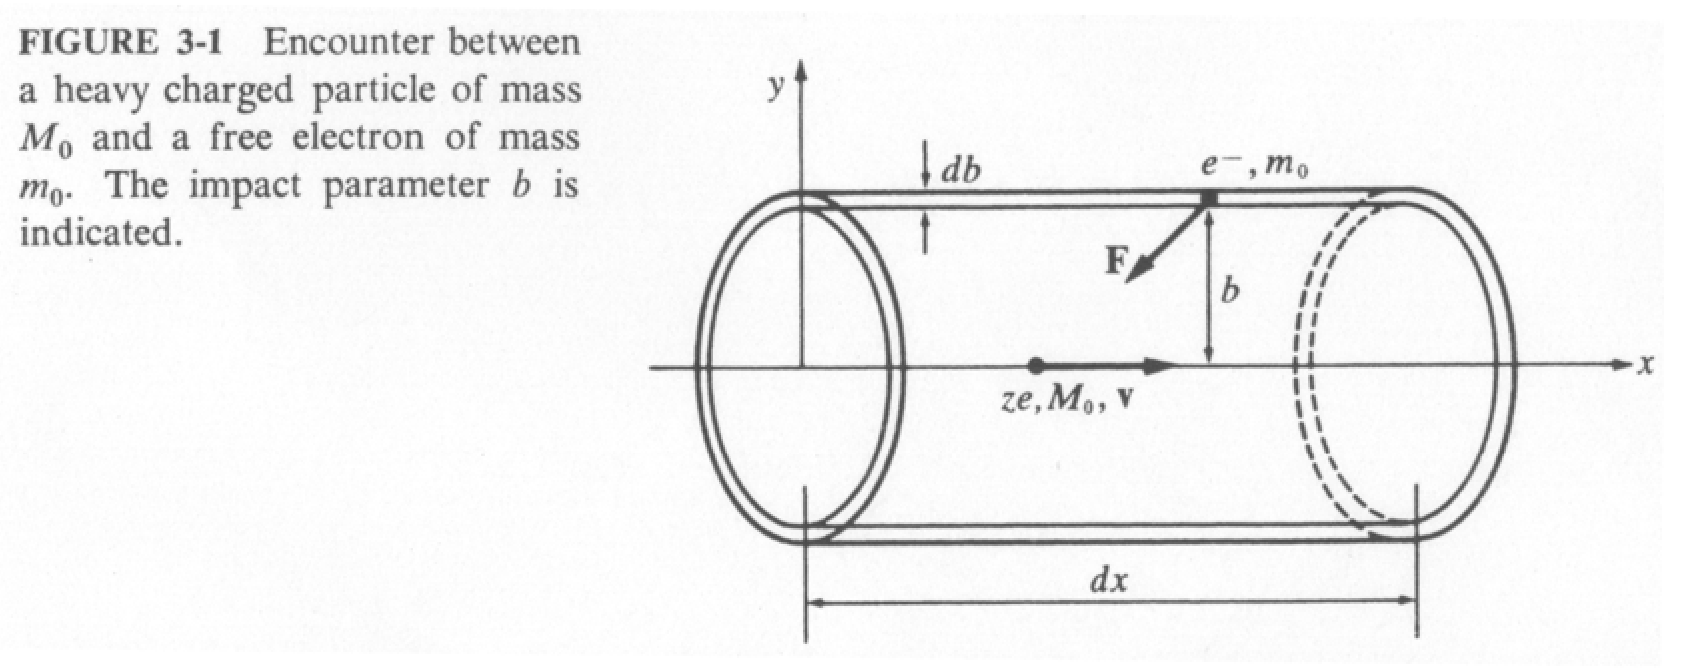
\includegraphics[width=4in]{images/ni/cp-collision.png}
  \caption{Collision Cylinder for Deriving the Energy Loss} \label{cp-collision}
\end{figure}

\begin{align}
    P_e &= \int \dt \overbrace{\frac{Ze^2}{x^2 + b^2}}^{F} \overbrace{\frac{b}{\sqrt{x^2 + b^2}}}^{\cos \theta} \\
    &= \int_{-\infty}^{\infty} \frac{2e^2}{x^2+b^2} \frac{b}{\sqrt{x^2 + b^2}} \frac{\dx}{v} \\
    &\approx \frac{2e^2 b}{v} \int \frac{\dx}{(x^2 + b^2)^{3/2}} = \frac{2Ze^2}{vb} \\
    \frac{P_e^2}{2m} &= \frac{2 (Ze^2)^2}{m_e b^2 v^2} 
\end{align}
Then we can write the energy loss per distance $\dTdx$, using that $2 \pi b \derivative b \dx$ is the element volume, $\left(\frac{Zze^2}{v b} \right)^2 \frac{1}{2m_e}$ is the energy loss, $n$ is the number density in \#/$\cm^3$, and $nZ$ is the number of neutrons per volume, 
\begin{align}
    \mbox{Stopping Power} &= - \frac{\dT}{\dx} = \int_{b_{min}}^{b_{max}} (2 \pi b \derivative b) \frac{1}{2m_e} \left( \frac{Zze^2}{vb} \right)^2 (n Z) \\
    &= \frac{4 \pi (Ze^2)^2nZ }{m_e v^2 } \ln \left( \frac{b_{max}}{b_{min}} \right) = \frac{4 \pi Z^2 e^4 n Z}{m_e v^2} \ln \left( \frac{2 m_e v^2}{\bar{I}} \right) 
\end{align}
A word about the $\frac{b_{max}}{b_{min}}$: we need to estimate this term; fortunately, a log function changes slowly, so we do not care all that much about the accuracy of this term. We estimate it as $\frac{2m_e v^2}{I}$. 

Relativistic Stopping Power, `Bethe Formula' (correction for high energy):
\eqn{\left( -\dTdx \right)_{\mathrm{coll}} = \frac{4 \pi Z^2 e^4 nZ}{m_e v^2} \left[ \ln \left( \frac{2 m_e c^2 \beta^2}{I (1-\beta^2) } \right) - \beta^2 \right]   }
collision with nucleus: $\left( -\dTdx \right)_{\mathrm{coll}}$ increases by factor of Z; decreases by factor of $\frac{m_e}{M[Z]}$. 

The take-away is, 
\eqn{ \Aboxed{ \left( -\dTdx \right)_{\mathrm{coll}} &\propto \frac{nZ}{m} } }
\subtopic{Radiation Loss, Range}
The radiation loss is not all that interesting; but the range is important! We start by defining radiation loss as emission of x-rays due to sudden deceleration of charged particles. We do a hand-wavy argument about intensity (which is always the square of another quantity): 
\eqn{ I \sim (ze \times \mathrm{acceleration})^2 \sim \left( \frac{zeZe}{m} \right)^2 }
That is, \hi{radiation loss is important for high Z absorber with a small mass (e.g., electrons matter, radiation loss does not matter for heavy charged particles).} 
After derivation (see SY6), we arrive at 
\eqn{ \left( - \dTdx \right)_{\mathrm{rad}} = n \int_0^T \d(hv) hv \left[ \frac{\dsigma}{\derivative (hv)} \right]_{\mathrm{rad}} = n (T+ m_e c^2) \sigma_{\mathrm{rad}} \boxed{\sim (T + m_e c^2) }  } 


\begin{align}
    R &= \int_0^R \dx = \int_{E_0}^0 \frac{\dx}{\dE} \dE = \int_0^{E_0} \left( - \frac{\dE}{\dx} \right)^{-1} \dE 
\end{align}
In the $\frac{1}{v^2}$ range, $R \sim \int_0^{E_0} E \dE = E_0^2$. 
In the log/real range, $R\ sim \int_0^{E_0} \dE  = E_0$. 
A good rule of thumb to remember about comparing two particles' range:
\eqn{ \frac{R_1 (v)}{R_2 (v)} = \frac{Z_2^2 M_1}{Z_1^2 M_2} }

Range of validity:
\begin{itemize}
    \item $E \gg 500 \bar{I}$. 
    \item $\frac{Z e^2}{\hbar v} = \left( \frac{e^2}{\hbar c} \right) \frac{Z}{v/c} = \frac{Z}{137 (v/c) } \ll 1 $
\end{itemize}



%%%% 
\subtopic{Mass absorption} 
\eqn{ - \dTdx \sim nZ = \frac{\rho N_0}{A} Z = \rho N_0 \frac{Z}{A} }
If we consider $\frac{Z}{A}$ to be a constant, then this seems to imply that stopping power divided by density is a constant for all matter. That is, if we define $\dw = \rho \dx$, then $-\frac{\dT}{\dw}$ should be constant. See Fig.14.1. 


%%%%%%%%%%% 
\subtopic{Cerenkov Radiation}
Typically, $v_{light} = \frac{c}{n}.$ For instance, speed of light in water is 0.75c. When $v> \frac{c}{n}$, we see the blue glow in ractors that are water cooled. 



\subtopic{Summary}
\begin{enumerate}
\item Compare the electron curve to the proton curve, it looks like the proton curve is just electron curve shifted to the right (shifted to higher energies). 
\item Know that $m_p = 2000 m_e$, so for the same set-up, the collision loss for protons is 2000 times that of electrons. 
\item It is safe to ignore radiation loss for protons; whereas for electrons we have to consider both collision loss and radiation loss. 
\end{enumerate}

\begin{figure}[ht]
  \centering
  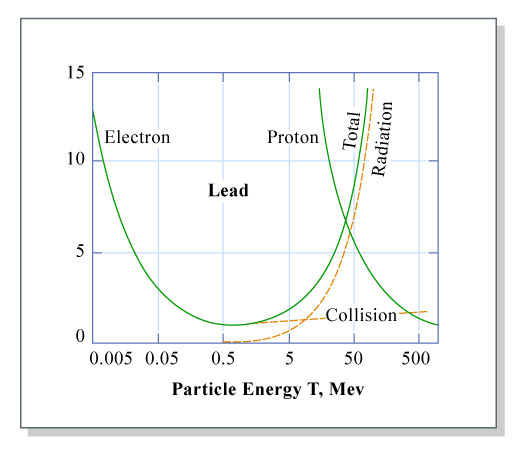
\includegraphics[width=5in]{images/ni/lead-ep.png}
  caption{Electron and Proton Energy Loss in Lead}
\end{figure}


%\begin{figure}
%   \centering
%   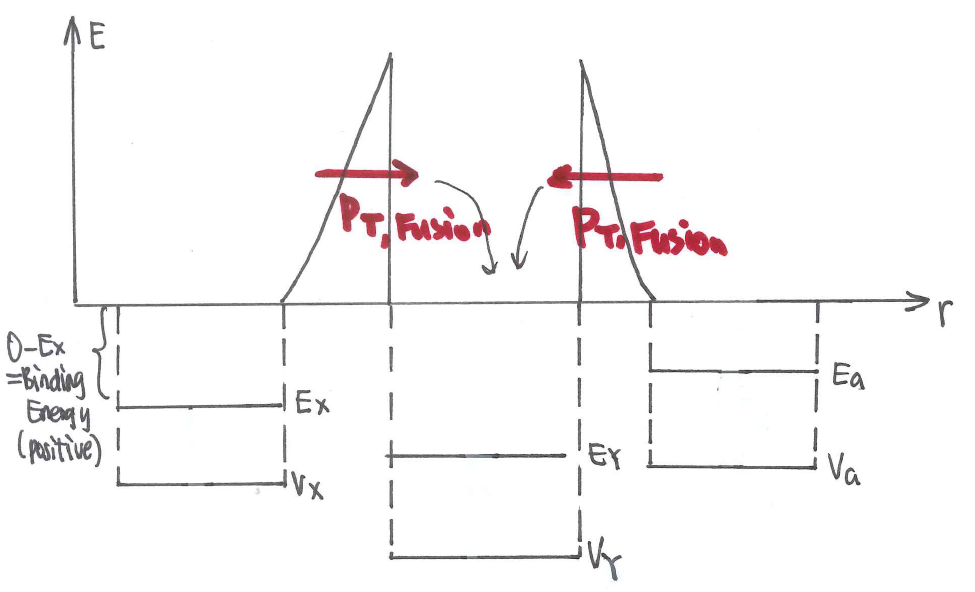
\includegraphics[width=4in]{images/ni/fusion-mechanism.png}
%   \caption{Mechanism for Fusion\label{fusion-mechanism}}
%\end{figure}



\end{document}
